\documentclass [a4paper,12pt,oneside,final]{article}
\usepackage[left=15mm,top=15mm,right=15mm,bottom=20mm]{geometry}
\usepackage{tikz}
\usepackage{float}
\usepackage{subfig}
\usetikzlibrary{matrix,chains,positioning,decorations.pathreplacing,arrows,arrows,shapes.geometric}

\title{%
Redes Neuronales \\
Trabajo Final \\
CNET \\
}
\date{2020}
\author{Igor Andruskiewitsch}

\begin{document}
    \maketitle

\section{Introducción}

En este trabajo vamos a ver la estructura y lógica detrás de construir una red neuronal artificial ({\it ANN}) desde cero con el objetivo de automatizar las clasificación de dígitos del dataset MNIST.

Vamos a analizar la arquitectura y los hiperparámetros utilizados, los resultados obtenidos y algunas particularidades de la implementación. No vamos a analizar el algoritmo de optimización ni su implementación, por cuestiones de simplicidad, aunque si vamos a explicar las singularidades y limitaciones que presentó la implementación.

\subsection{Objetivos}

\begin{itemize}
    \item{Explicar el diseño y la arquitectura}
    \item{Listar las limitaciones}
    \item{Describir la arquitectura de red utilizada para clasificar dígitos del {\it MNIST}}
    \item{Visualizar los resultados del punto anterior}
\end{itemize}

\section{Diseño}

El diseño que elegimos para la implementación de nuestra red neuronal, se basa en dos componentes:

\begin{itemize}
    \item{{\bf cnet} es un contenedor para nuestra red, contiene la información de {\it entrada/salida} y nuestras capas}
    \item{{\bf clayer} representa cada una de las capas de nuestra red, almacena:}
        \begin{itemize}
            \item{una matriz de {\it pesos}}
            \item{un arreglo de {\it tendencias} (bias)}
            \item{un tipo de {\it activación} (limitadas en la implementación)}
            \item{un arreglo llamado {\it delta}, que contiene pasos intermedios del algoritmo de backprop}
            \item{un arreglo {\it output}, que contiene el último vector que dió como resultado la capa}
        \end{itemize}
\end{itemize}

También definimos otros módulos, que nos permiten manipular con facilidad los datos resultantes o las funciones necesarias durante el entrenamiento de nuestro modelo.

\begin{itemize}
    \item{{\bf cnet\_loss\_type} define los tipos de {\it pérdidas} soportadas, para las cuales se define una implementación y su derivada:}
        \begin{itemize}
            \item{{\it mse\_loss} (Error Medio Cuadrado)}
            \item{{\it cross\_entropy\_loss} (Entropía Cruzada)}
        \end{itemize}
    \item{{\bf cnet\_act\_type} define los tipos de {\it activaciones} soportadas, para las cuales se define una implementación y su derivada:}
        \begin{itemize}
            \item{{\it relu\_act} (ReLU)}
            \item{{\it sigmoid\_act} (Sigmoide para clasificación binaria)}
            \item{{\it softmax\_act} (Softmax para clasificación con multiples clases)}
        \end{itemize}
\end{itemize}

\section{Limitaciones}

En esta sección vamos a desarrollar algunas de las limitaciones con las que contamos a la hora de desarrollar la librería

\subsection{Algoritmo de backprop}

El algoritmo elegido para actualizar los pesos de nuestra red es el {\bf GD}{\it (Gradiente Descendiente Simple)}. Esto significa que no vamos a utilizar batches (lotes) para inferir con nuestro modelo como se hace con el {\bf SGD}(Gradiente Descendiente Estocástico). Esto se debe a la complejidad agregada de variar la forma del input a tomar por nuestro modelo, simplificamos esta variable utilizando un único input. Esta decisión trae consigo algunos puntos en contra, ya que es necesario dedicar más épocas de entrenamiento, aunque vemos que cada época representa una caída en la pérdida, a diferencia del {\it SGD}, que puede variar generando caídas o subidas en la pérdida en cada época.

\subsection{Capas disponibles}

Otra limitación a considerar son las capas disponibles, que en este caso son únicamente {\bf capas neuronales}, es decir que no contamos con {\bf dropout}, {\bf convoluciones} ni otros tipos de capa. Esto significa que no podemos utilizar la librería para realizar análisis sobre imágenes complejas (por eso la utilización del {\it MNIST}). También es necesario tener cuidado con los hiperparámetros para evitar el {\it sobreajuste}, ya que no contamos con la capa de {\bf dropout} para ajustar estos valores.

\subsection{Hiperparámetros y optimizaciones}

Para nuestra librería, el algoritmo de entrenamiento cuenta con parámetros limitados, sólo podemos proveer el {\it learning rate} y la cantidad de {\it épocas}. No contamos con un método para realizar {\it weight decay}, ni {\it momentum}. Estos métodos podrían generar un entrenamiento mucho más certero pero no se incluyeron para evitar complejizar la librería.

\section{Clasificación de {\it MNIST}}

En esta sección vamos a explicar la arquitectura que elegimos para un modelo que clasifique los dígitos del dataset {\it MNIST}. Esta es una tarea de clasificación de múltiples clases, ya que el dataset cuenta con dígitos entre $0$ y $9$ y queremos que nuestro modelo sea capaz de predecir, dada la imágen, a qué digito corresponde. A primera vista, la mejor arquitectura incluiría capas convolucionales, en conjunto con un output activado por la función {\it Softmax}, que limita la suma de las probabilidades a $1$ y una función de pérdida de {\it Entropía Cruzada}. En nuestro caso, vamos a utilizar la función de activación {\it Sigmoide}, que limita cada probabilidad a un número en $0$ y $1$, y como función de pérdida, vamos a tener la función {\it MSE}. Si bien no es la combinación ideal para la tarea, veremos que obtuvimos resultados bastante buenos.


La arquitectura capa por capa de la red es la siguiente:

\begin{figure}[htp]
\centering
\tikzset{%
  every neuron/.style={
    circle,
    draw,
    minimum size=1cm
  },
  neuron missing/.style={
    draw=none, 
    scale=4,
    text height=0.333cm,
    execute at begin node=\color{black}$\vdots$
  },
}

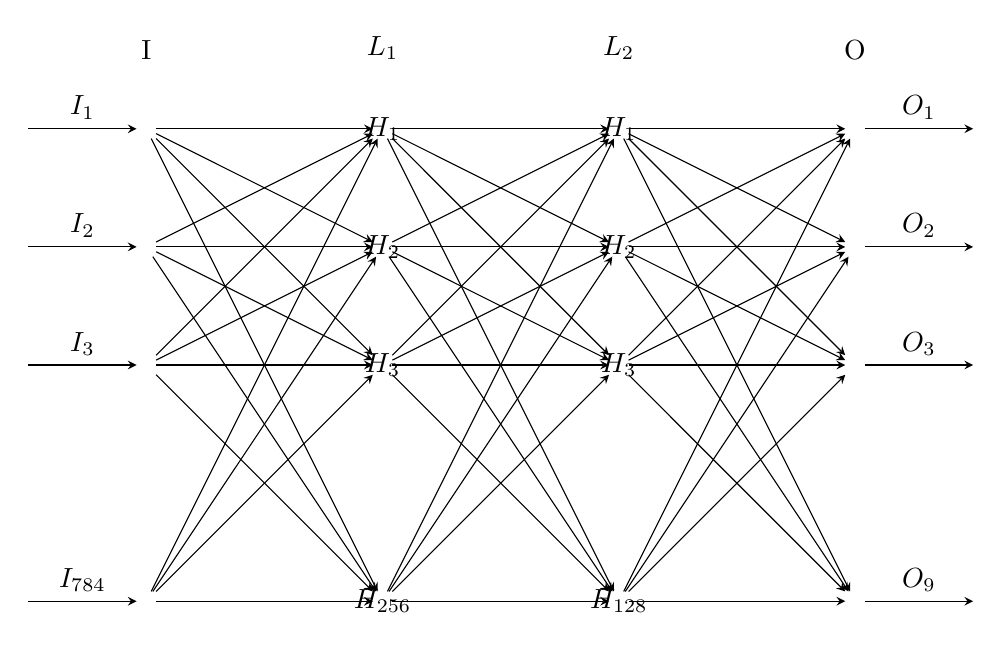
\begin{tikzpicture}[x=1.5cm, y=1.5cm, >=stealth]

\foreach \m/\l [count=\y] in {1,2,3,missing,4}
  \node [every neuron/.try, neuron \m/.try] (input-\m) at (0,2.5-\y) {};

\foreach \m [count=\y] in {1,2,3,missing,4}
  \node [every neuron/.try, neuron \m/.try ] (hidden-1-\m) at (2,2.5-\y) {};

\foreach \m [count=\y] in {1,2,3,missing,4}
  \node [every neuron/.try, neuron \m/.try ] (hidden-2-\m) at (4,2.5-\y) {};

\foreach \m [count=\y] in {1,2,3,missing,4}
  \node [every neuron/.try, neuron \m/.try ] (output-\m) at (6,2.5-\y) {};

\foreach \l [count=\i] in {1,2,3,784}
  \draw [<-] (input-\i) -- ++(-1,0)
    node [above, midway] {$I_{\l}$};

\foreach \l [count=\i] in {1,2,3,256}
  \node [align=center] at (hidden-1-\i) {$H_{\l}$};

\foreach \l [count=\i] in {1,2,3,128}
  \node [align=center] at (hidden-2-\i) {$H_{\l}$};

\foreach \l [count=\i] in {1,2,3,9}
  \draw [->] (output-\i) -- ++(1,0)
    node [above, midway] {$O_{\l}$};

\foreach \i in {1,...,4}
  \foreach \j in {1,...,4}
    \draw [->] (input-\i) -- (hidden-1-\j);

\foreach \i in {1,...,4}
  \foreach \j in {1,...,4}
    \draw [->] (hidden-1-\i) -- (hidden-2-\j);

\foreach \i in {1,...,4}
  \foreach \j in {1,...,4}
    \draw [->] (hidden-2-\i) -- (output-\j);

\foreach \l [count=\x from 0] in {I, $L_1$, $L_2$, O}
  \node [align=center, above] at (\x*2,2) {\l};

\end{tikzpicture}
\caption{Arquitectura para nuestro modelo de clasificación.}\label{fig:nn}
\end{figure}

Vemos que tenemos un input de tamaño $784$, que las imágenes del {\it MNIST} son de $28 x 28$, tenemos dos capas ocultas de tamaño $256$ y $128$ respectivamente, y recibimos como salida un vector de tamaño $10$, con las probabilidades correspondientes para la clasificación de los dígitos del $0$ al $9$.


\section{Resultados {\it MNIST}}

La arquitectura descripta en la sección anterior fue entrenada por 200 épocas. Este proceso tardó aproximadamente unas 5 horas.

\begin{figure}%
    \centering
    \subfloat[]{{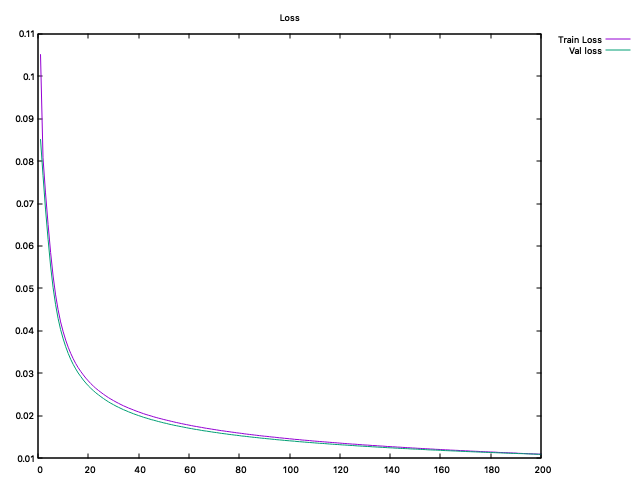
\includegraphics[width=8cm]{./graficos/mnist_losses.png} }}
    \qquad
    \subfloat[]{{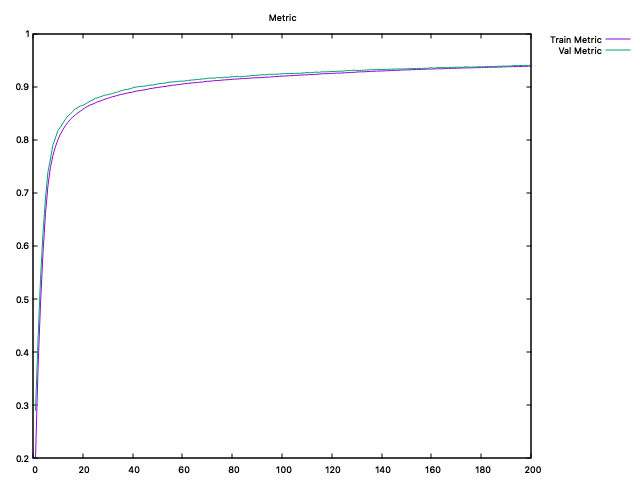
\includegraphics[width=8cm]{./graficos/mnist_metrics.png} }}
    \caption{Métricas de entrenamiento}\label{fig:mnist_metrics}
\end{figure}

Podemos observar en la figura \ref{fig:mnist_metrics} que las curvas de las métricas de los datos validación y entrenamiento no tienen grandes diferencias, por lo que podríamos pensar que no hubo sobreajuste. La pérdida y la exactitud finales del modelo fueron de aproximadamente $0.01$ y $0.94$ respectivamente.

Una vez terminado el entrenamiento, también se realizaron tests sobre los datos de prueba. De estas pruebas, obtuvimos la siguiente matriz de confusión 

\begin{figure}[ht]
  \centering
  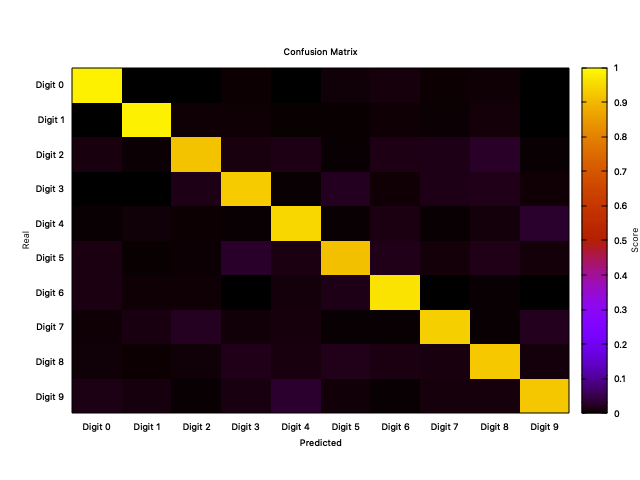
\includegraphics[width=13cm,keepaspectratio]{./graficos/mnist_conf_matrix.png}
  \caption{Matriz de confusión para los datos de validación del MNIST}\label{fig:mnist_conf_matrix}
\end{figure}

En esta podemos observar que la gran mayoría de los dígitos fueron clasificados correctamente, aunque hubo algunos dígitos clasificados incorrectamente. Para comprender mejor cuáles son los dígitos que generan problemas en nuestro modelo, generamos un reporte de clasificación, que incluye distintas métricas:

\begin{verbatim}
         precision  recall     f1-score   support 
Digit 0  0.951533   0.981633   0.966349   980 
Digit 1  0.973753   0.980617   0.977173   1135 
Digit 2  0.948744   0.914729   0.931426   1032 
Digit 3  0.931480   0.928713   0.930094   1010 
Digit 4  0.925224   0.945010   0.935013   982 
Digit 5  0.928981   0.909193   0.918980   892 
Digit 6  0.933131   0.961378   0.947044   958 
Digit 7  0.947628   0.932879   0.940196   1028 
Digit 8  0.919140   0.921971   0.920554   974 
Digit 9  0.936492   0.920714   0.928536   1009 

Final Accuracy: 0.940300 - Samples: 10000
\end{verbatim}

En este reporte podemos observar que, a excepción del $0$ y el $1$, la mayoría de los dígitos tienen métricas menores a $9.5$, esto puede deberse a que el $0$ y el $1$ son más dígitos comunes en dataset (la métrica {\bf support} del reporte es de los datos de validación y no de entrenamiento). Aún así las métricas son buenas, no bajan de $0.9$ y podrían mejorarse utilizando técnicas no soportadas mencionadas anteriormente.

\end{document}
